\documentclass[10pt]{article}
\usepackage[margin=0.75in]{geometry}\usepackage[T1]{fontenc}\usepackage{amsmath,amssymb,tikz}
\begin{document}\section*{Ordered B-zero route: composed preservation}
\textbf{Producer result; independent fidelity review pending.}

The exact ordered \texttt{sameUDouble} dispatcher and literal $B=0$ derive $s\ne0$. Composing that guard with the retained word-level point extraction and doubling theorem yields canonical extracted coordinates, a nonzero extracted ordinate, a selected doubled payload with canonical coordinates and nonzero weights, and normalized Mumford validity. Unlike the earlier payload theorem, this composition does not assume $s\ne0$ separately.

\begin{center}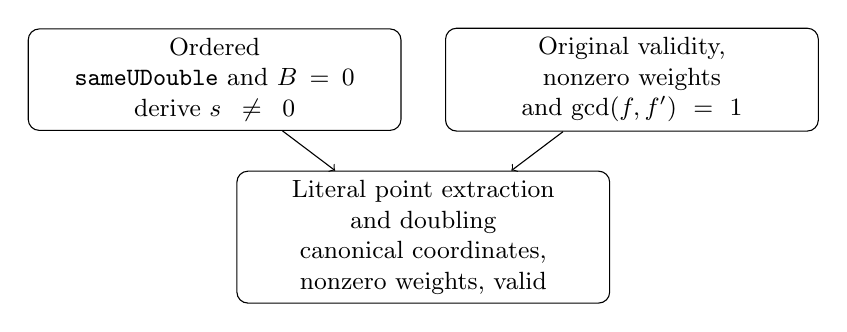
\begin{tikzpicture}[every node/.style={draw,rounded corners,align=center,text width=4.5cm,minimum height=1.1cm,font=\small}]
\node (g) at (0,0) {Ordered \\ \mbox{\texttt{sameUDouble}} and $B=0$\\derive $s\ne0$};
\node (p) at (5.3,0) {Original validity, nonzero weights\\and $\gcd(f,f')=1$};
\node (o) at (2.65,-2) {Literal point extraction\\and doubling\\canonical coordinates,\\nonzero weights, valid};
\draw[->] (g)--(o);\draw[->] (p)--(o);
\end{tikzpicture}\end{center}
\subsection*{Assumptions and statement boundary}
Prime $5\le p<2^{31}$; twelve canonical input coordinates; four canonical curve coefficients; degree-one arithmetic without lookup tables. The curve is the monic quintic without an $X^4$ term. Input $a$ has normalized Mumford validity and nonzero $z,w$; the polynomial and its derivative are coprime. Input $b$ supplies the exact crossed-coordinate dispatch; no additional validity or nonzero-weight premise about $b$ is consumed.

This is the selected B-zero helper route. It does not formalize all other \texttt{add22} returns or prove a divisor-class-sum statement, compiler behavior, or operation counters. The imported BZero and word-guard producer packets retain their pending independent-review status.
\subsection*{Fixed original-input check}
For $p=5$, coefficients $(a_0,a_1,a_2,a_3)=(0,4,1,0)$, choose
\[
a=(1,0,4,0,2,3),\qquad b=(4,0,1,0,1,1)
\]
in $(q,r,s,t,z,w)$ order. They use different coordinate scales. The outer classifier returns \texttt{sameUDouble}, $B=0$, the extracted $(x,y,z,w)$ is $(4,4,3,3)$ and the doubled output is
\[
(q,r,s,t,z,w)=(2,1,3,2,3,3).
\]
The complete composed proposition is applied without an $s\ne0$ argument. Original normalized validity and the explicit polynomial Bezout certificate are reused from the byte-preserved field fixture module.

Six new fixed propositions also check the earlier inverse branch for zero ordinates, a same-double input with $B=3$ outside this lemma, and exclusion of $p=2$. These are fixed proof controls, not a cohort or a timing experiment.
\subsection*{Evidence and next step}
The main declarations, copied fixture module, new controls and separate axiom readback have individual command and input-binding receipts. \texttt{status.json} records their exact outcomes. \texttt{control-data.json} contains typed inputs and outputs; \texttt{flow.svg} is the editable diagram. No new cost ratio is assigned. Independent source and statement review precedes canonical integration.

Sources: retained \texttt{projective\_law\_gate.rs}, lines 727--753 and 911--935; \texttt{PROOF\_AUDIT.md}; guard, BZero field, and WordBZero producer packets. The composition adds no new arithmetic formula.
\end{document}
